% pdflatex HLA.tex
\documentclass[12pt]{article}

\usepackage{fullpage}
\usepackage{multicol, multirow}
\usepackage{tabularx}
\usepackage{graphicx}
\usepackage{ulem}
\usepackage[utf8]{inputenc}
\usepackage[russian]{babel}

\begin{document}

\begin{titlepage}

\newpage

% insert a title page here

\end{titlepage}
\tableofcontents{}



\newpage
\section{Высокоуровневая архитектура}
\subsection{Концепция}
% Короткий рассказ о системе
Программа интернет-мессенджер для социальной сети <<Вконтакте>>. Программа позволит отправлять и принимать текстовые сообщения пользователям из списка друзей, подгружать историю сообщений с сервера, а также уведомлять о новых сообщениях с помощью всплывающих окон.

\subsection{Физическая архитектура}
% Диаграмма
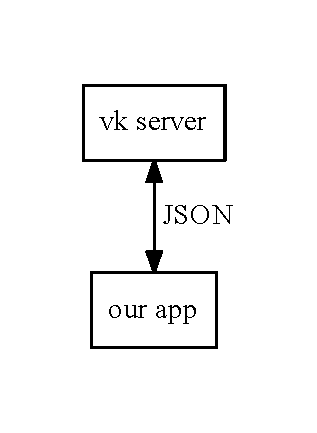
\includegraphics{../HLA/diag/phys.pdf}

\subsection{Логическая архитектура}
% Описание модулей и их взаимодействия, диаграмма
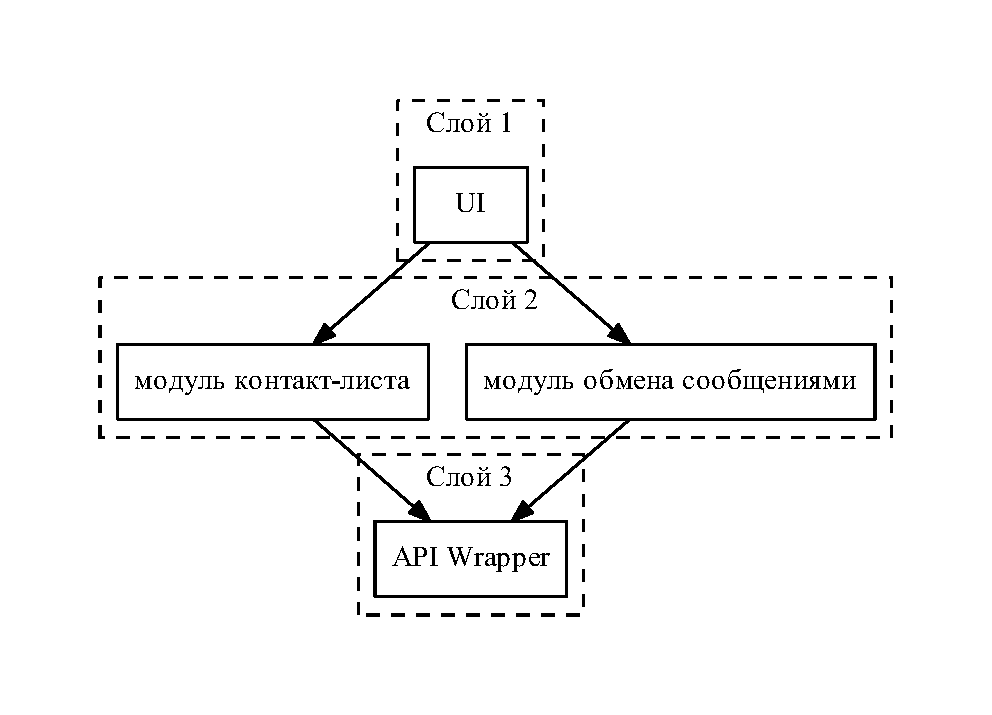
\includegraphics{../HLA/diag/logic.pdf}

\subsection{Нефункциональные требования}
% Требования, накладывающиеся на какие-то свойства системы

\subsubsection*{Производительность}
Время отправки/получения сообщений, если они есть на сервере, при стабильном интернет-соединении (ping до vk.com < 100 ms) — в диапазоне от 1 до 2 c.

\subsubsection{Сопровождаемость}
Самодокументируемый код, комментарии к неочевидным моментам. Логгирование ошибок в консоли Python. \\
Доступен репозиторий на GitHub (http://github.com/r3t/oop-project), где можно оставлять сообщения об ошибках и недочётах

\subsubsection{Пользовательский интерфейс}
Интерфейс минималистичен, требуемые подписи к элементам управления — на английском.

\subsubsection{Операционное окружение}
Кроссплатформенность: Windows, Linux, Mac OS и любая другая система, позволяющая работать с графическим интерфейсом и имеющая интерпретатор языка Python.

\subsubsection{Безопасность}
Пароль пользователя нигде не хранится ни в явном, ни в шифрованном виде.

\subsection{Компоненты и инструменты} 
\begin{enumerate}
\item Python 2.7.X
\item PyQt 4.10.3+
\item vkontakte 1.3.2 (vk.com (aka vkontakte.ru) API wrapper)
\end{enumerate}



\newpage
\section{Распределение ролей}
\subsection{Ильвохин Дмитрий}
\begin{itemize}
\setlength{\itemsep}{-1mm} % уменьшает расстояние между элементами списка
\item Диаграммы HLA
\item Интерфейс и логика работы главного окна
\item Интерфейс и логика работы окна логина
\item Интерфейс и логика работы всплывающих окон
\item Работа с API
\item Работа с потоками
\item Реализация шаблонов <<Реестр>>, <<Фасад>> и обработки ошибок (шаблон <<Декоратор>>)
\end{itemize}

\subsection{Данилычев Иван}
\begin{itemize}
\setlength{\itemsep}{-1mm}
\item Интерфейс и логика работы окна и вкладок сообщений
\item Интерфейс и логика работы окна настроек
\item Функционал окна сообщений
\item Ресурсы приложения (иконки)
\end{itemize}


\newpage
\section{Примененные шаблоны проектирования}
\subsection{Реестр}
В реестре (класс {\tt Registry}) хранятся единичные экземпляры объектов, к которым требуется доступ из, возможно, любого модуля. Такими объектами стали:
\begin{itemize}
\setlength{\itemsep}{-1mm} % уменьшает расстояние между элементами списка
\item Конфигурация приложения. Она существует в единственном числе, при этом, помимо главного окна, требуется во вкладках сообщений и, собственно, самого окна настроек.
\item Обертка над классом, работающим с API, поскольку клиент сообщений однопользовательский.
\end{itemize}

\subsection{Фасад}
Фасад (класс {\tt VkClientThread}) служит посредником между обёрткой и главным окном. Он хранит в себе результаты последних запросов к API, а также распределяет их по компонентам приложения с помощью потоков, каждый из которых отвечает за свои типы запросов. Таким образом, фасад снимает постоянную или частую нагрузку с интерфейса, позволяя пользователю работать с приложением.

\subsection{Декоратор}
Декоратор, представленный классом {\tt exception\_handling}, выступает в виде надстройки над перехватчиком исключений. % прозреваю, что на самом деле ещё и над фасадом

\section{Схема работы класса Vk Thread Client}
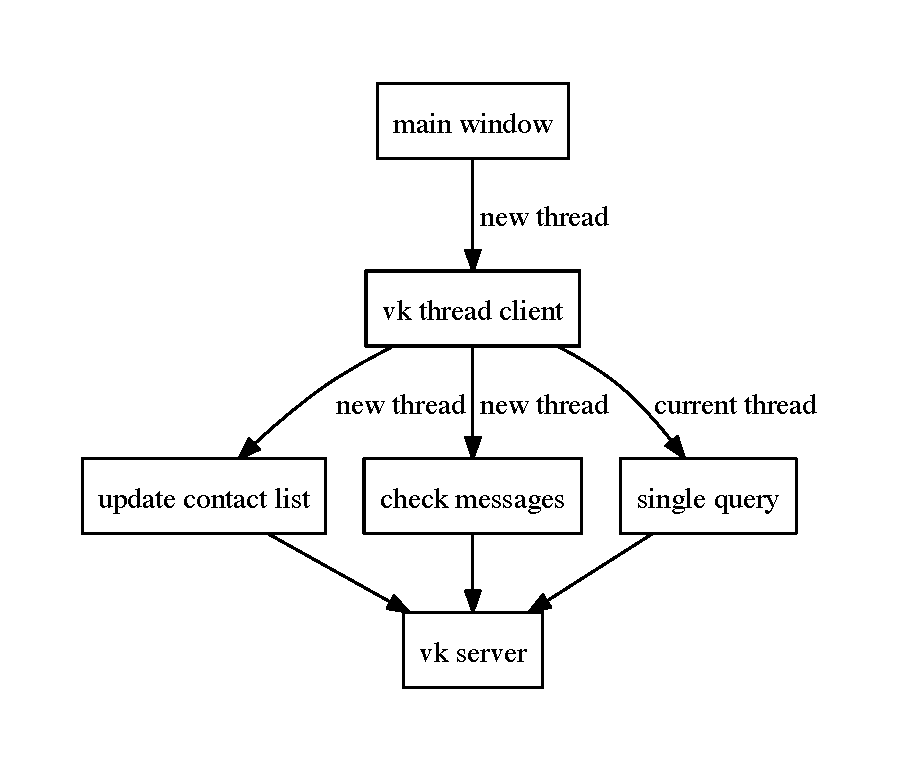
\includegraphics{./diag/work_logic.pdf}

\newpage
\section{Модульное тестирование}
\subsection{Инструменты}
% TODO: fill in

\subsection{Тесты}
% TODO: fill in

% тест для проверки сохранения и записи файла конфига
% тест для проверки парсера ссылок
% тест для ещё чего-нибудь? Не уверен, что у нас есть ещё компонент, вывод которого можно с чем-нибудь подиффать



\newpage
\section{Функциональное тестирование}
\subsection{Тест-кейс 1}
% TODO: fill in

% сценарий проверки получения и отправки сообщений
% сценарий проверки уведомлений: звук и иконки
% сценарий проверки создания новых (и не очень) вкладок



\newpage
\section{Выводы}
\indent При разработке клиента сообщений очень пригодились такие шаблоны проектирования, как реестр и фасад: первый упростил взаимодействие между классами, избавив их, а заодно и разработчиков, от проблемы постоянного обмена одними и теми же объектами и контроля их единственности. Фасад облегчил работу со сторонней библиотекой, объединив запросы к серверу и контроль актуальности получаемых ответов. Кроме того, за счёт некоторого усложнения логики фасада была облегчена логика основного приложения: фасад сам сигнализирует о наличии необходимых данных, используя концепцию сигналов и слотов библиотеки (Py)Qt. \newline

На проектировании и логике работы сильно сказалась зависимость от сервера. Первоначальная версия приложения при любом запросе к API ВКонтакте <<замораживала>> интерфейс, в связи с чем потребовались отдельные потоки для запросов. Помимо нашего мессенджера, к серверу подключается множество других пользователей, в связи с чем некоторые потоки время от времени получают вместо реального ответа сообщение о таймауте запроса (и не только). Чтобы связь не терялась неявно, был написан отдельный класс-декоратор, устанавливающий соединение и передающий его дальше по коду, обрабатывая таким образом исключения. Кроме того, он выводит в консоль лог пойманных исключений. \newline

Повлияло наличие сервера также и на процесс тестирования. Поскольку контролировать получаемые данные, как и эмулировать работу сервера, оказалось затруднительно, основная работа пришлась на тестирование функционала приложения и составление тест-кейсов. Модульное тестирование было проведено лишь для немногих самостоятельных внутренних компонентов, к примеру, разметке ссылок в окне чата.
\end{document}
